\section{Results}
\label{sec:results}

All results are Spectre simulations of the schematic at \SI{27}{\celsius} and
$\Vdd=\SI{1.8}{\volt}$ through the course testbench, in the five corners TT,
SS, FF, SF and FS.

\subsection{Transfer and resolution across corners}
\label{sec:corners}

Figure~\ref{fig:staircase} shows the measured transfer with one fixed trim
configuration (the trimmed TT setting) in all five corners; Table~\ref{tab:corners}
lists the extracted metrics. Every corner produces a monotonic 31-step
staircase with an intact thermometer code, and every corner passes the
\SI{20}{\pico\second} requirement, with the slowest corner (SS,
\SI{18.2}{\pico\second}) closest to the limit. The skewed corners SF and FS
barely differ from TT because opposite N and P shifts largely cancel in an
inverter pair. The input-referred offset stays between $-7$ and
\SI{-24}{\pico\second}, constant per corner: a code offset, not a linearity
error.

\begin{figure}[htb]
\centering
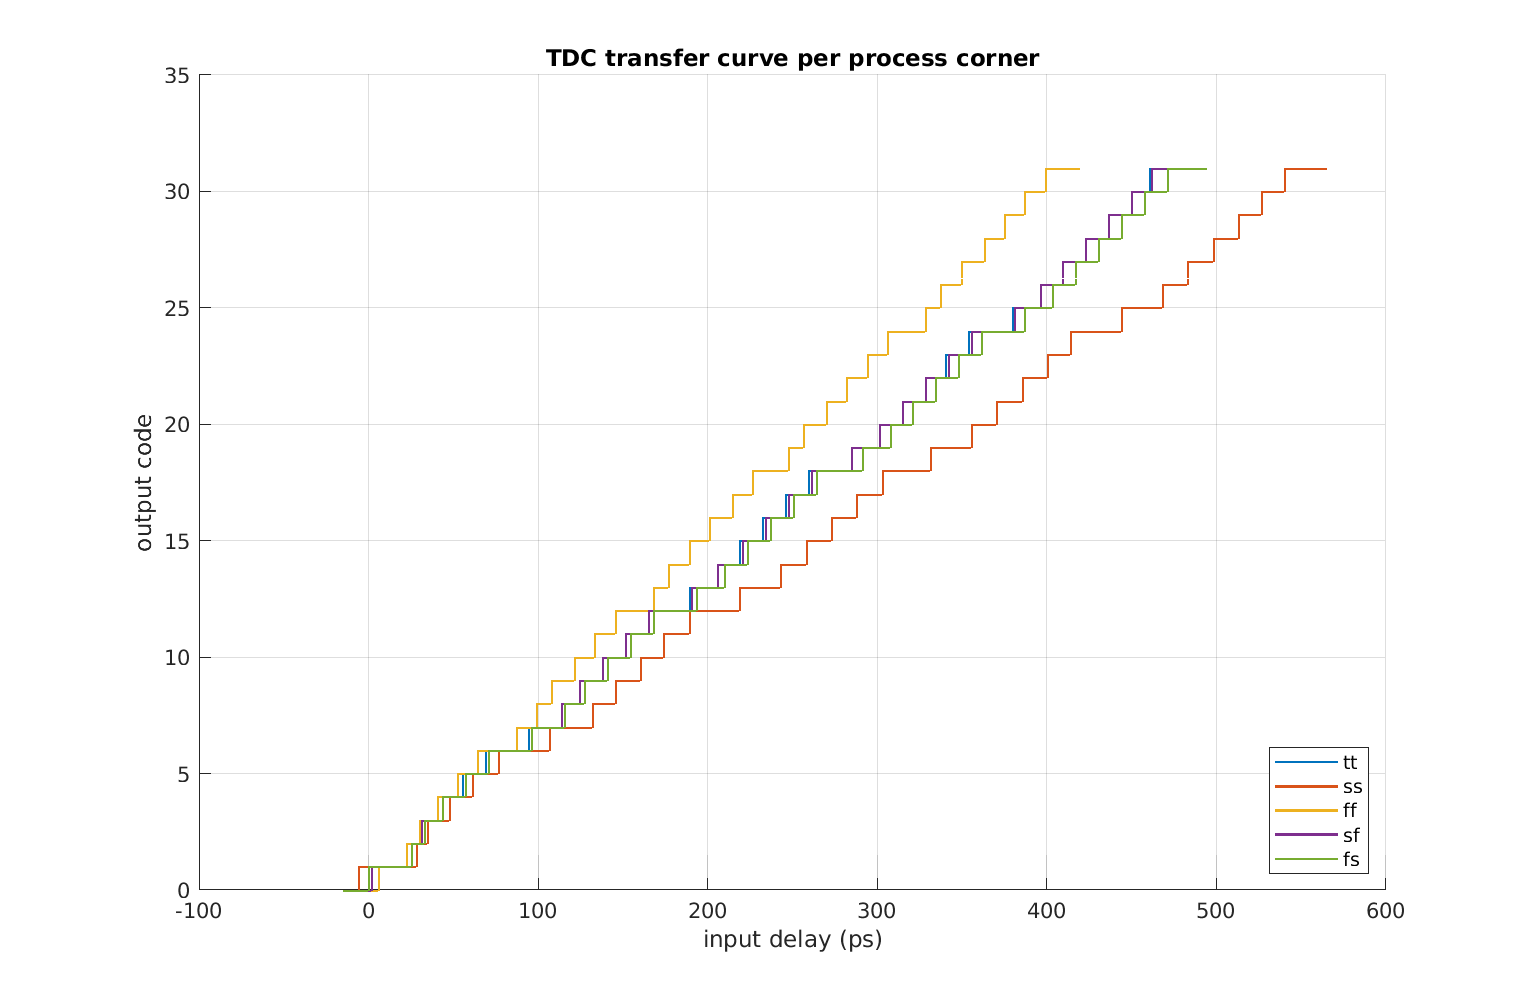
\includegraphics[width=0.72\textwidth]{figures/staircase_all_corners.png}
\caption{TDC transfer per corner, fixed trim configuration. All corners are
monotonic and reach code 31; the slope spreads with corner speed.}
\label{fig:staircase}
\end{figure}

\begin{table}[H]
\centering
\small
\caption{Corner results with one fixed trim configuration. INL is the course
half-range convention; energy and FoM from the supply-ammeter measurement.
Every corner passes all sign-off checks (no missing codes, monotonic,
LSB below \SI{20}{\pico\second}).}
\label{tab:corners}
\begin{tabular}{l S[table-format=2.2] S[table-format=1.2] S[table-format=1.2] S[table-format=-2.1] S[table-format=2.2] S[table-format=1.2] S[table-format=1.2]}
\toprule
\textbf{Corner} & {\textbf{LSB}} & {\textbf{DNL$_{\max}$}} &
{\textbf{INL}} & {\textbf{Offset}} &
{\textbf{E/conv}} & {\textbf{ENOB}} & {\textbf{FoM}} \\
 & {(\si{\pico\second})} & {(LSB)} & {(LSB)} & {(\si{\pico\second})} &
{(\si{\pico\joule})} & {(bit)} & {(\si{\pico\joule}/step)} \\
\midrule
TT & 15.35 & 0.66 & 0.65 & -15.4 & 11.67 & 4.54 & 0.50 \\
SS & 18.20 & 0.90 & 0.76 & -24.2 & 10.76 & 4.39 & 0.51 \\
FF & 13.10 & 0.72 & 0.58 & -7.1  & 12.84 & 4.58 & 0.54 \\
SF & 15.35 & 0.66 & 0.61 & -13.9 & 11.96 & 4.57 & 0.50 \\
FS & 15.70 & 0.72 & 0.61 & -15.7 & 11.38 & 4.56 & 0.48 \\
\bottomrule
\end{tabular}
\end{table}

\subsection{Linearity}
\label{sec:linearity}

\begin{figure}[htb]
\centering
\begin{subfigure}[t]{0.49\textwidth}
  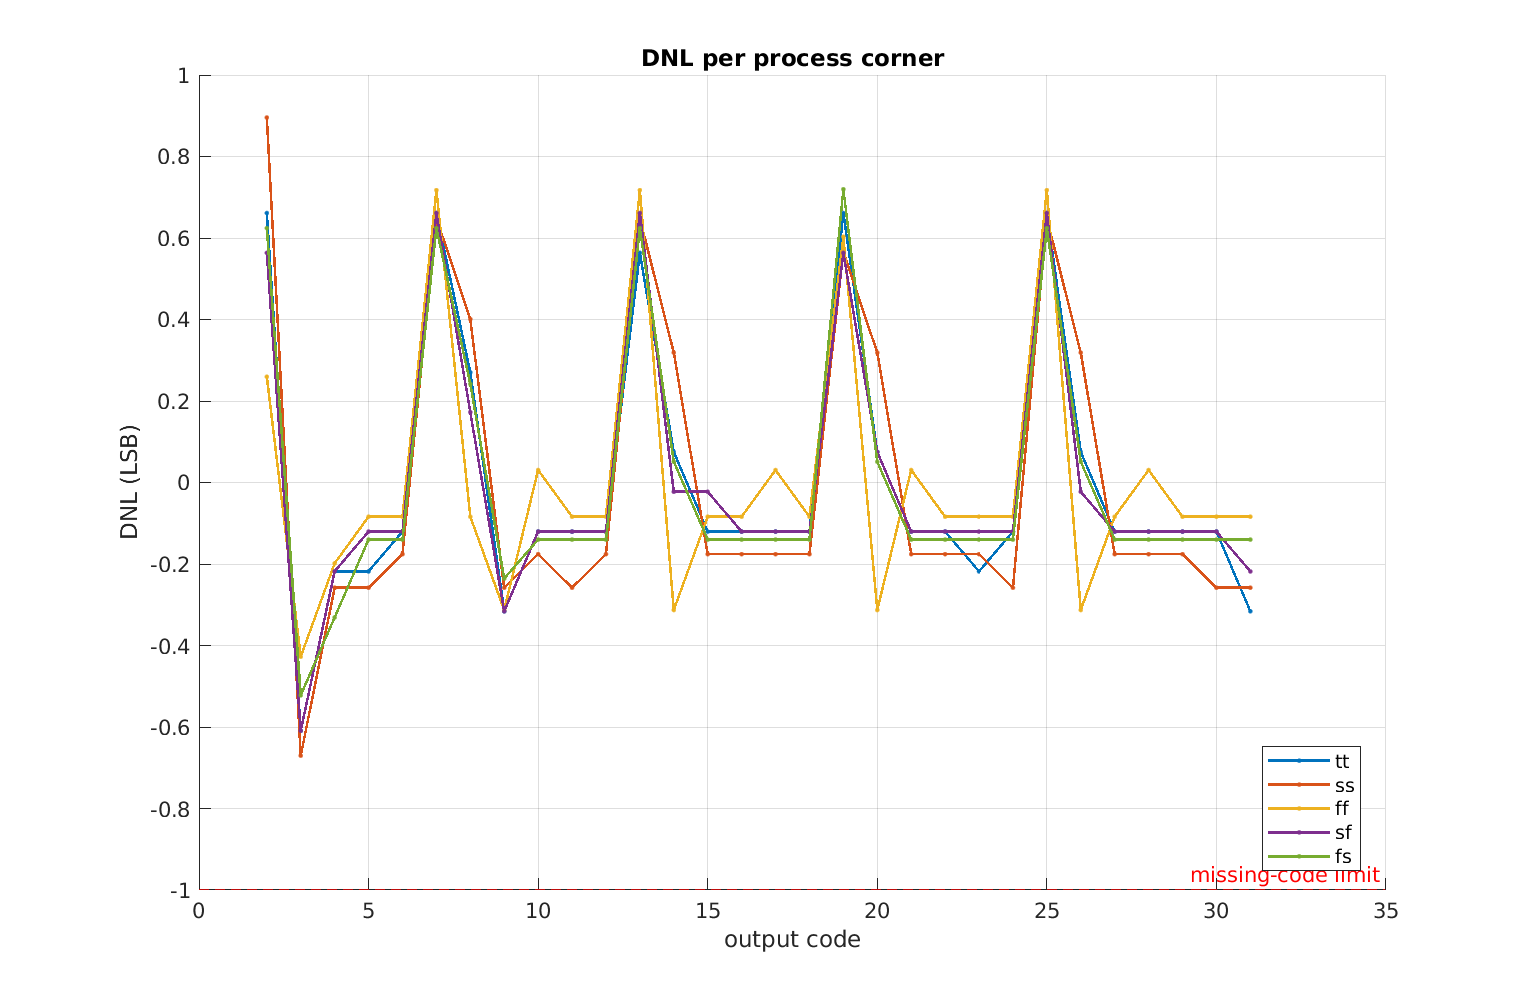
\includegraphics[width=\textwidth]{figures/dnl_per_corner.png}
  \caption{DNL per corner.}
  \label{fig:dnl}
\end{subfigure}\hfill
\begin{subfigure}[t]{0.49\textwidth}
  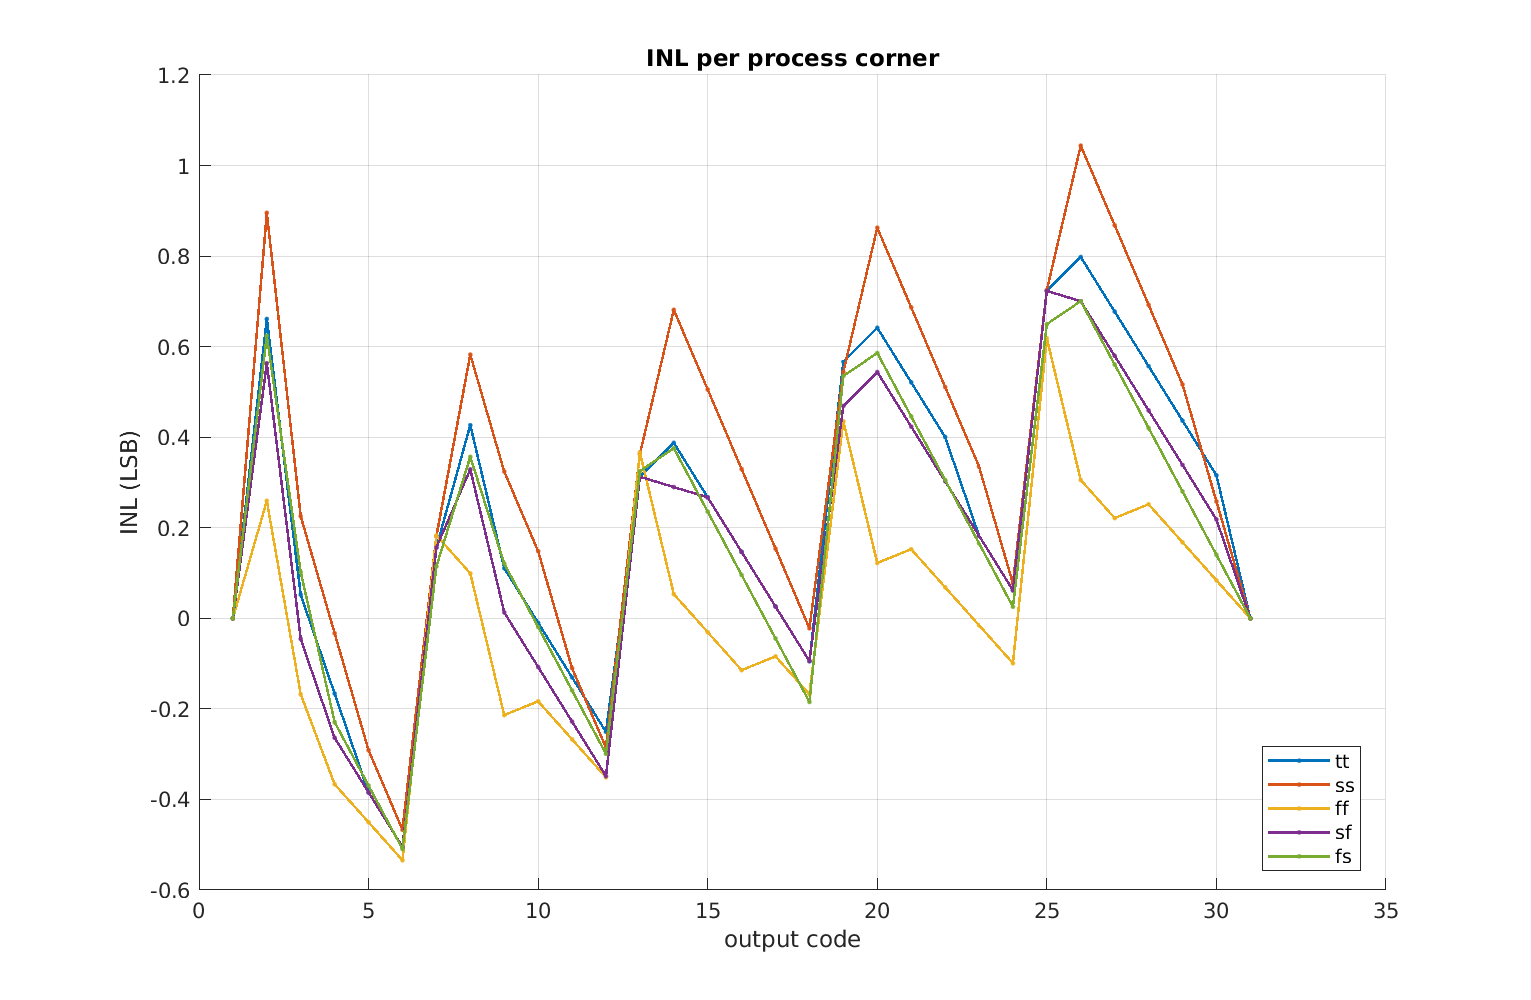
\includegraphics[width=\textwidth]{figures/inl_per_corner.png}
  \caption{INL per corner (endpoint convention).}
  \label{fig:inl}
\end{subfigure}
\caption{Linearity with fixed trim. The period-6 sawtooth marks the column-wrap
boundaries of the $k=6$ mapping and repeats identically in every corner.}
\label{fig:linearity}
\end{figure}

Worst-case DNL is \num{0.90} LSB (SS), well clear of the $-1$ LSB missing-code
limit; no corner loses a code (Fig.~\ref{fig:linearity}). Switching from the
half-range convention of Table~\ref{tab:corners} to the per-code endpoint
curve of Fig.~\ref{fig:inl}, the worst endpoint INL is \num{1.04} LSB (SS);
all other corners stay at or below \num{0.80}. The dominant DNL feature is a
sawtooth with period 6, peaking at \numrange{0.6}{0.7} LSB at codes 7, 13, 19
and 25: the column-wrap boundaries of the mapping in Eq.~\eqref{eq:mapping}.
The pattern is identical in every corner, so it is architectural rather than
mismatch-driven, and trimming cannot remove it
(Section~\ref{sec:calibration}). A targeted capacitive correction at the wrap
codes is listed as future work.

\subsection{Per-corner trimming}
\label{sec:calibration}

\begin{figure}[htb]
\centering
\begin{subfigure}[t]{0.49\textwidth}
  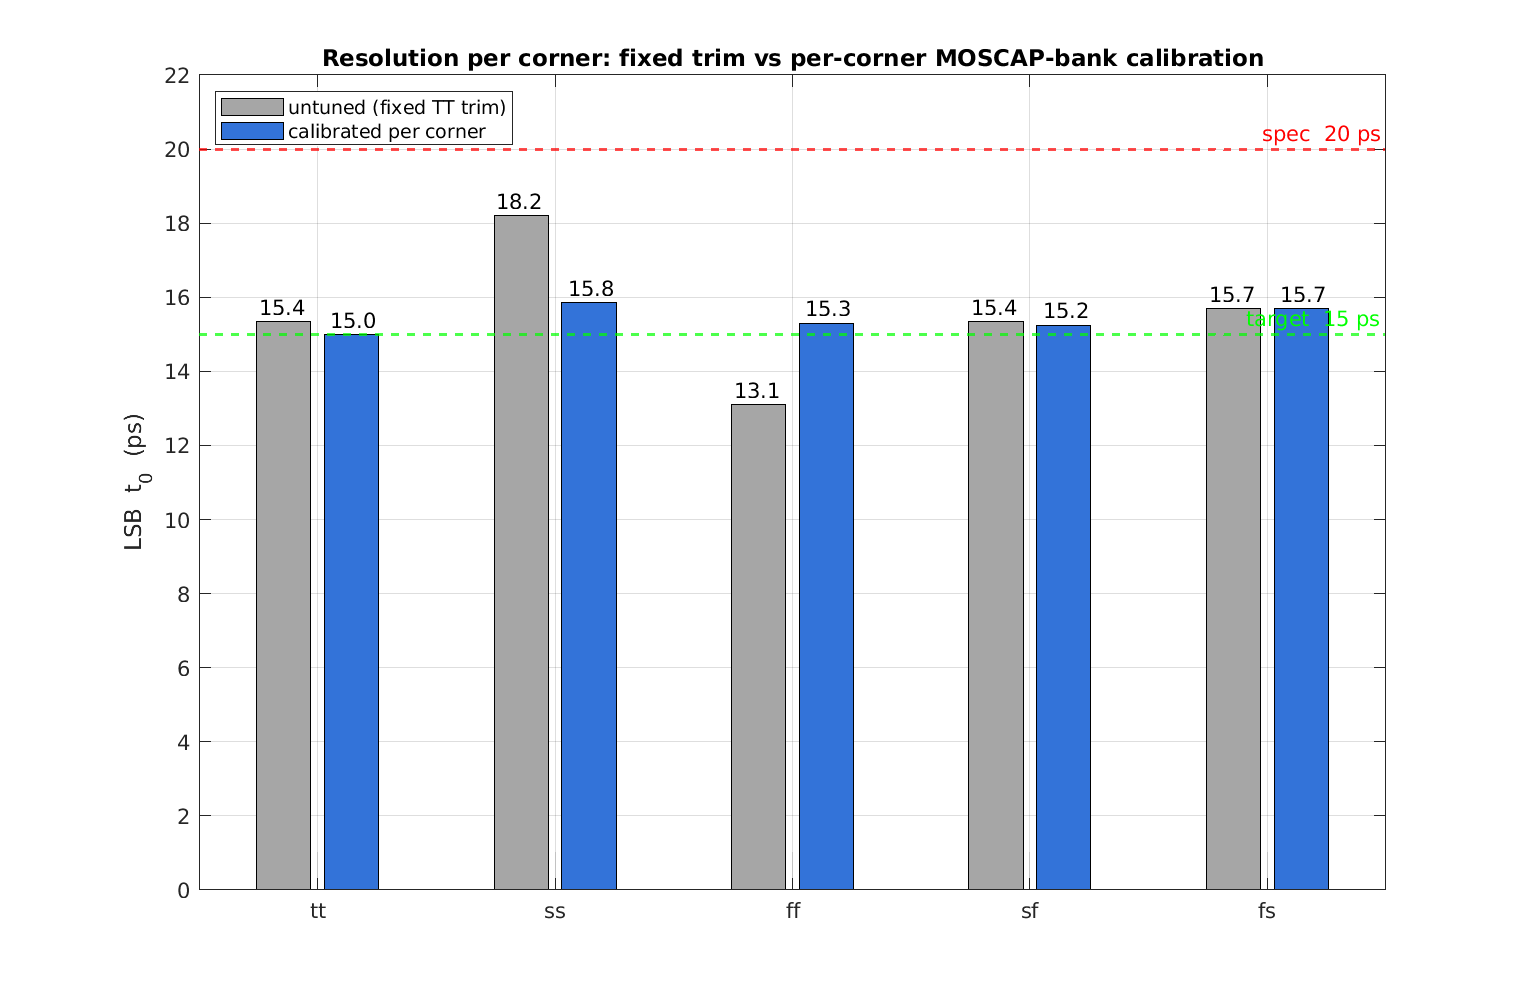
\includegraphics[width=\textwidth]{figures/lsb_tuned_vs_untuned.png}
  \caption{LSB per corner, fixed trim vs per-corner trim.}
  \label{fig:lsbtuned}
\end{subfigure}\hfill
\begin{subfigure}[t]{0.49\textwidth}
  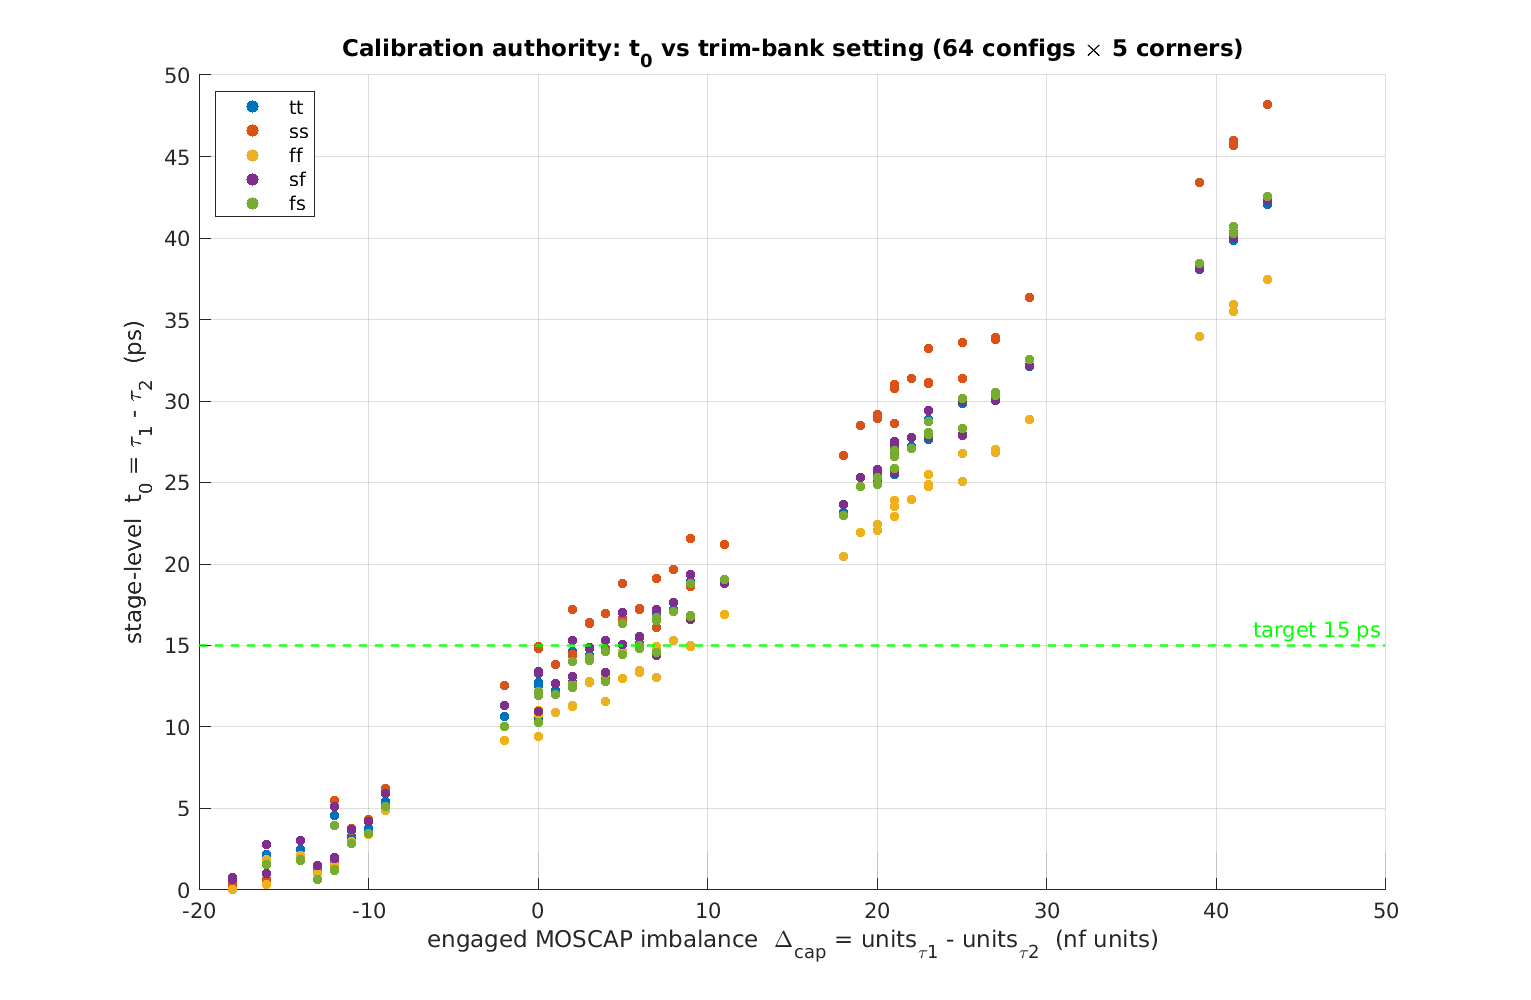
\includegraphics[width=\textwidth]{figures/calibration_range.png}
  \caption{Trim authority: stage-level $\tlsb$ vs engaged capacitance
  imbalance, all 64 configurations in 5 corners.}
  \label{fig:calrange}
\end{subfigure}
\caption{MOSCAP-bank trimming. Every corner re-centers to the
\SI{15}{\pico\second} target; the banks command roughly
\SIrange{0}{48}{\pico\second}, far more authority than the corners require.}
\label{fig:calfigs}
\end{figure}

Applying the per-corner trim codes of Appendix~\ref{app:trim} re-centers the
LSB to \SIrange{15.0}{15.85}{\pico\second}: the corner spread tightens from
\SI{5.10}{\pico\second} to \SI{0.85}{\pico\second}, six times, and the
worst-case margin to the specification grows from \num{1.8} to
\SI{4.15}{\pico\second} (Fig.~\ref{fig:lsbtuned}). DNL and INL barely move
(worst trimmed INL \num{0.74} LSB), consistent with the architectural origin
of the wrap pattern. All sign-off checks still pass in every corner.

\subsection{Energy, power and figure of merit}
\label{sec:energy}

\begin{figure}[htb]
\centering
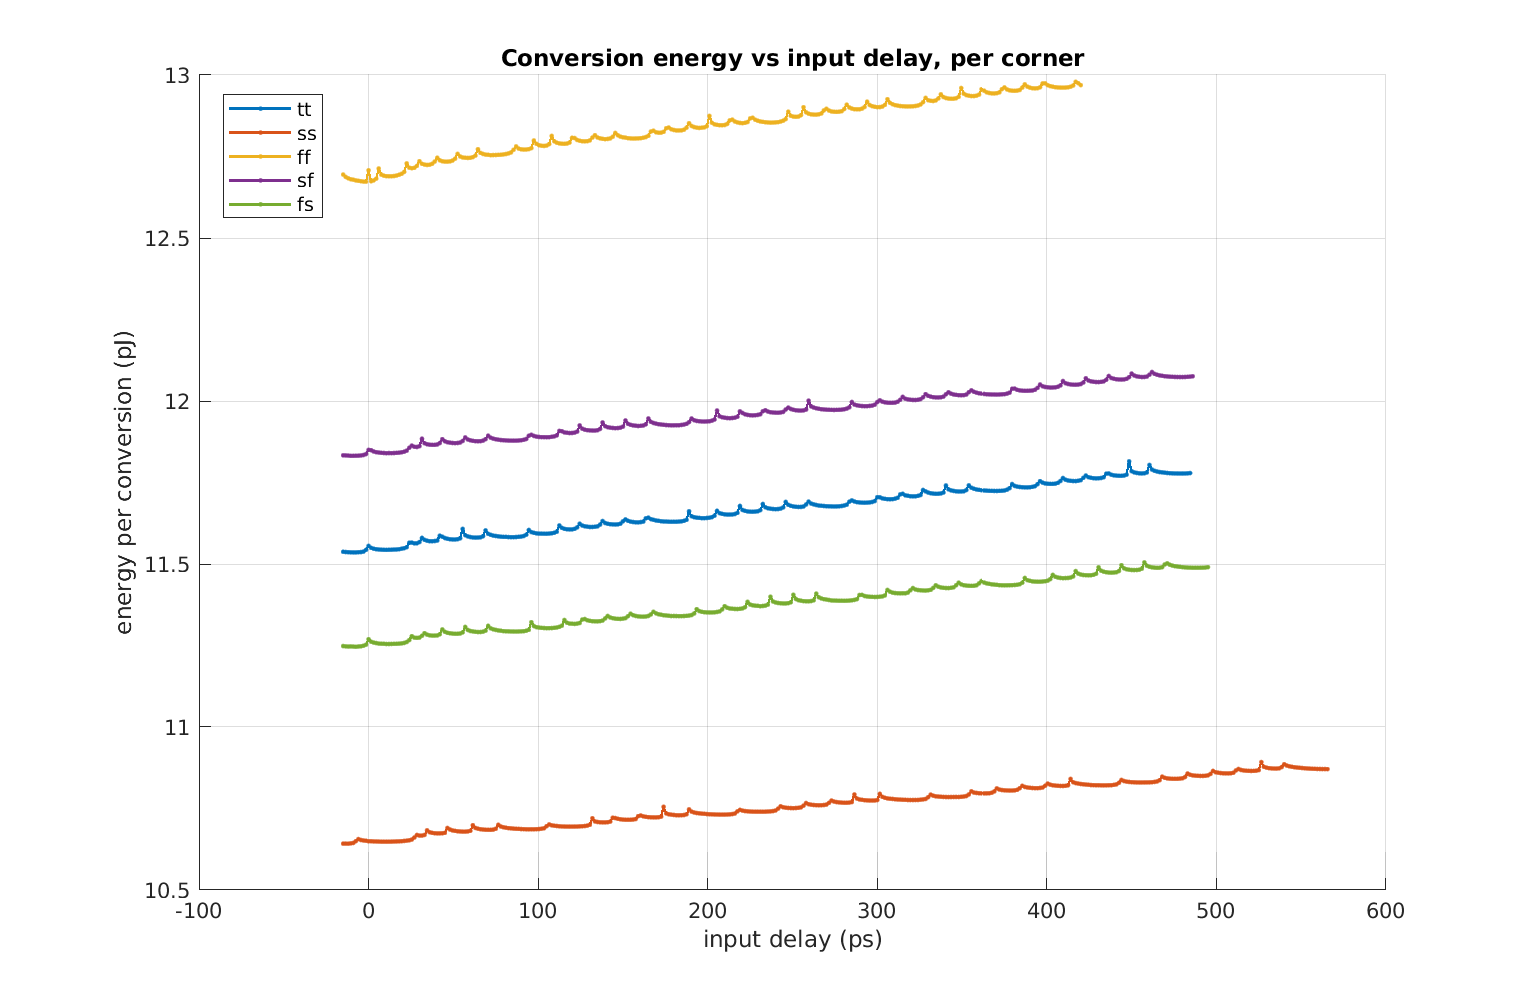
\includegraphics[width=0.62\textwidth]{figures/power_vs_delay.png}
\caption{Energy per conversion vs input delay, per corner. The band is nearly
flat; energy tracks corner speed.}
\label{fig:energy}
\end{figure}

Energy per conversion sits in a flat \SIrange{10.6}{13.0}{\pico\joule} band
across input delay and corner (Fig.~\ref{fig:energy}), ordered by corner speed
(SS lowest, FF highest). With the \SI{5}{\nano\second} conversion window of
the testbench this corresponds to an average power of
\SIrange{2.15}{2.57}{\milli\watt}. Table~\ref{tab:fom} reports both figure-of-merit
conventions: the specification's $P/\tlsb$ and the course script's
$E/2^{\mathrm{ENOB}}$. The dynamic range, $31\times\mathrm{LSB}$, spans
\SIrange{406}{564}{\pico\second} depending on the corner, with a
quantization-limited single-shot precision $\mathrm{LSB}/\sqrt{12}$ of
\SIrange{3.8}{5.3}{\pico\second}.

\begin{table}[H]
\centering
\small
\caption{Power and figure of merit per corner (fixed trim). $P_{avg}$ assumes
the \SI{5}{\nano\second} conversion window (\SI{200}{MS/s}).}
\label{tab:fom}
\begin{tabular}{l S[table-format=1.2] S[table-format=1.3] S[table-format=1.2]}
\toprule
\textbf{Corner} & {$P_{avg}$ (\si{\milli\watt})} & {$P/\tlsb$ (\si{\milli\watt}/\si{\pico\second})} & {$E/2^{\mathrm{ENOB}}$ (\si{\pico\joule}/step)} \\
\midrule
TT (nominal) & 2.33 & 0.152 & 0.50 \\
SS & 2.15 & 0.118 & 0.51 \\
FF & 2.57 & 0.196 & 0.54 \\
SF & 2.39 & 0.156 & 0.50 \\
FS & 2.28 & 0.145 & 0.48 \\
\bottomrule
\end{tabular}
\end{table}

\subsection{Area}
\label{sec:area}

The transistor-width total of the core is $\sumw = \SI{1305.6}{\micro\meter}$:
\SI{1078.3}{\micro\meter} of active width over 1120 devices plus
\SI{227.3}{\micro\meter} of MOSCAP over 65 devices, extracted from the Spectre
netlist. Including the testbench interface cells would
add \SI{93.7}{\micro\meter} (\texttt{TDC\_in} \SI{11.9}{\micro\meter},
\texttt{TDC\_out} \SI{81.8}{\micro\meter}). The per-cell breakdown is given in
Appendix~\ref{app:sigmaw}.

\subsection{Arbiter dead zone and metastability}
\label{sec:meta}

\begin{figure}[htb]
\centering
\begin{subfigure}[t]{0.49\textwidth}
  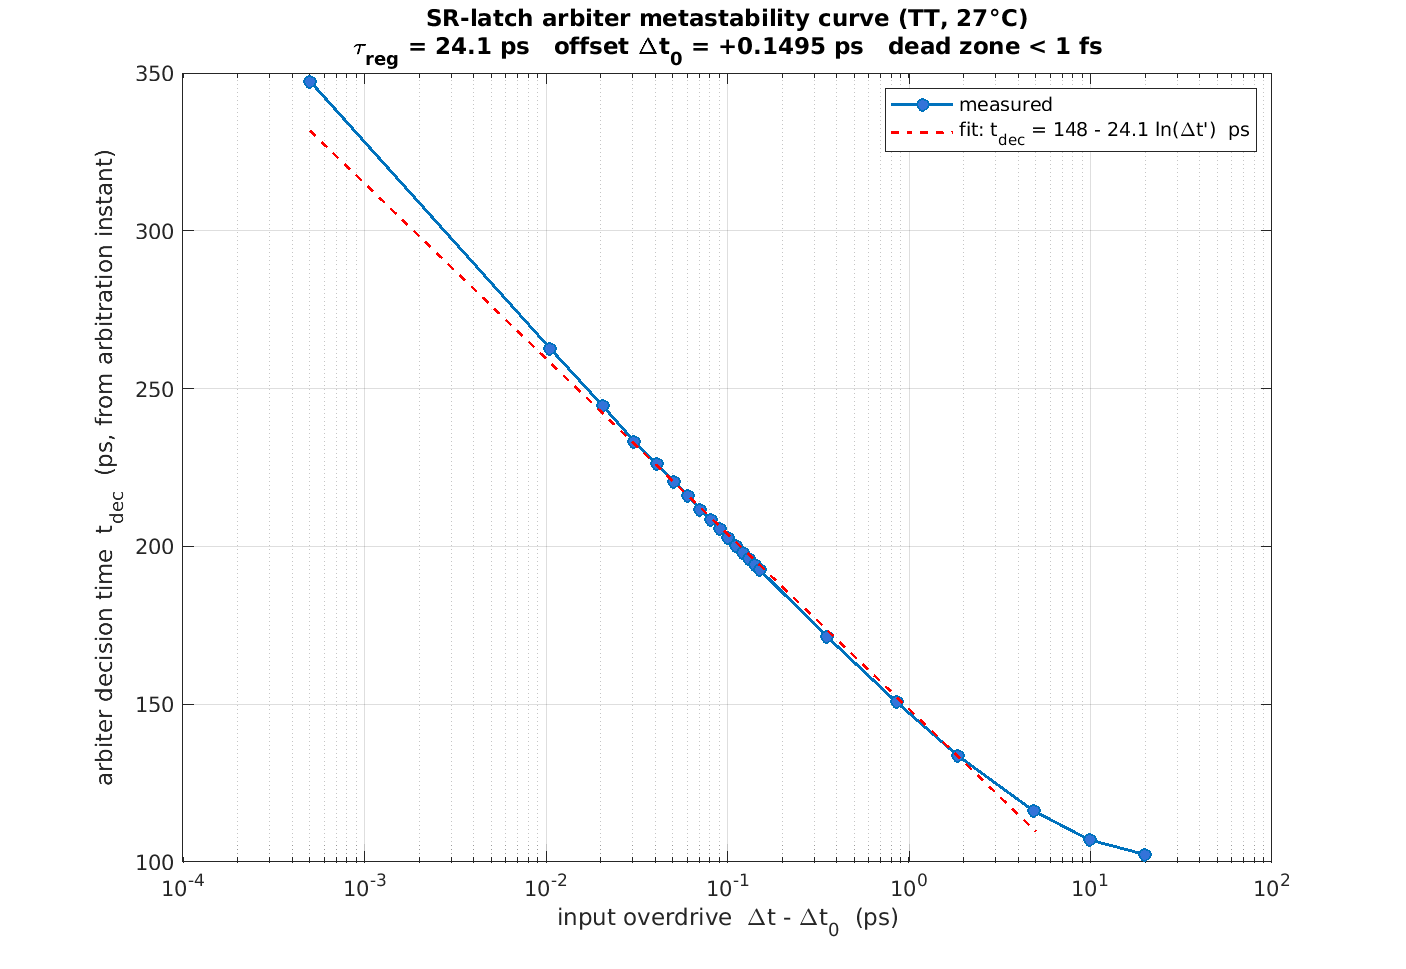
\includegraphics[width=\textwidth]{figures/metastability_curve.png}
  \caption{Decision time vs input overdrive.}
  \label{fig:metacurve}
\end{subfigure}\hfill
\begin{subfigure}[t]{0.49\textwidth}
  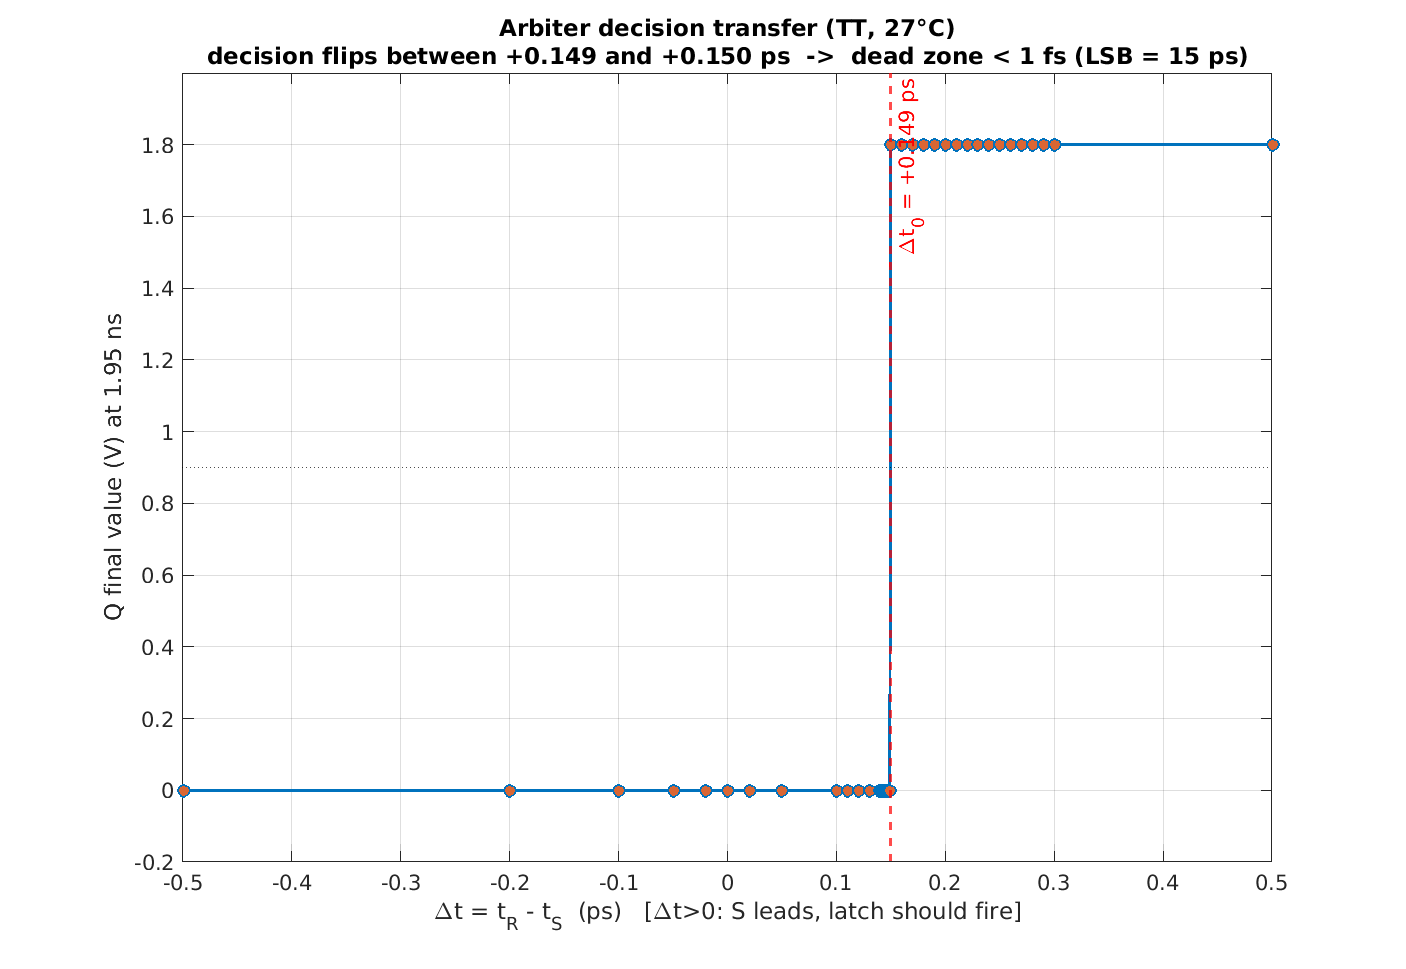
\includegraphics[width=\textwidth]{figures/deadzone_transfer.png}
  \caption{Final output vs $\dt$: the decision flips between adjacent
  \SI{1}{\femto\second} grid points.}
  \label{fig:deadzone}
\end{subfigure}
\caption{SR-latch arbiter characterization (TT, \SI{27}{\celsius},
\SI{5}{\femto\farad} loads), 49 simulations in three nested sweeps.}
\label{fig:meta}
\end{figure}

The smallest resolvable interval of the converter is set by the arbiter, so we
characterized it down to \SI{0.5}{\femto\second} of input overdrive
(Fig.~\ref{fig:meta}). The arbitration offset is
$\dt_0 = +149.5\pm\SI{0.5}{\femto\second}$, about 1\% of one LSB. The decision
time follows the classic regeneration law
$t_{dec} = t_{cq} + \tau_{reg}\ln(1/\dt')$ over three and a half decades with
$\tau_{reg}=\SI{24.1}{\pico\second}$ and a large-overdrive clk-to-Q of
\SI{102}{\pico\second}; the worst observed decision time is
\SI{347.5}{\pico\second} at \SI{0.5}{\femto\second} overdrive, still far
inside the conversion window. No ambiguous final value was observed anywhere
on the \SI{1}{\femto\second} grid, bounding the dead zone below
\SI{1}{\femto\second}, four orders of magnitude under the LSB. The bound is
grid-limited and noiseless (a Monte-Carlo analysis would widen it), which
still leaves orders of magnitude of margin.

\subsection{Measured comparison with a 1-D Vernier}
\label{sec:1dvs2d}

\begin{figure}[htb]
\centering
\begin{subfigure}[t]{0.49\textwidth}
  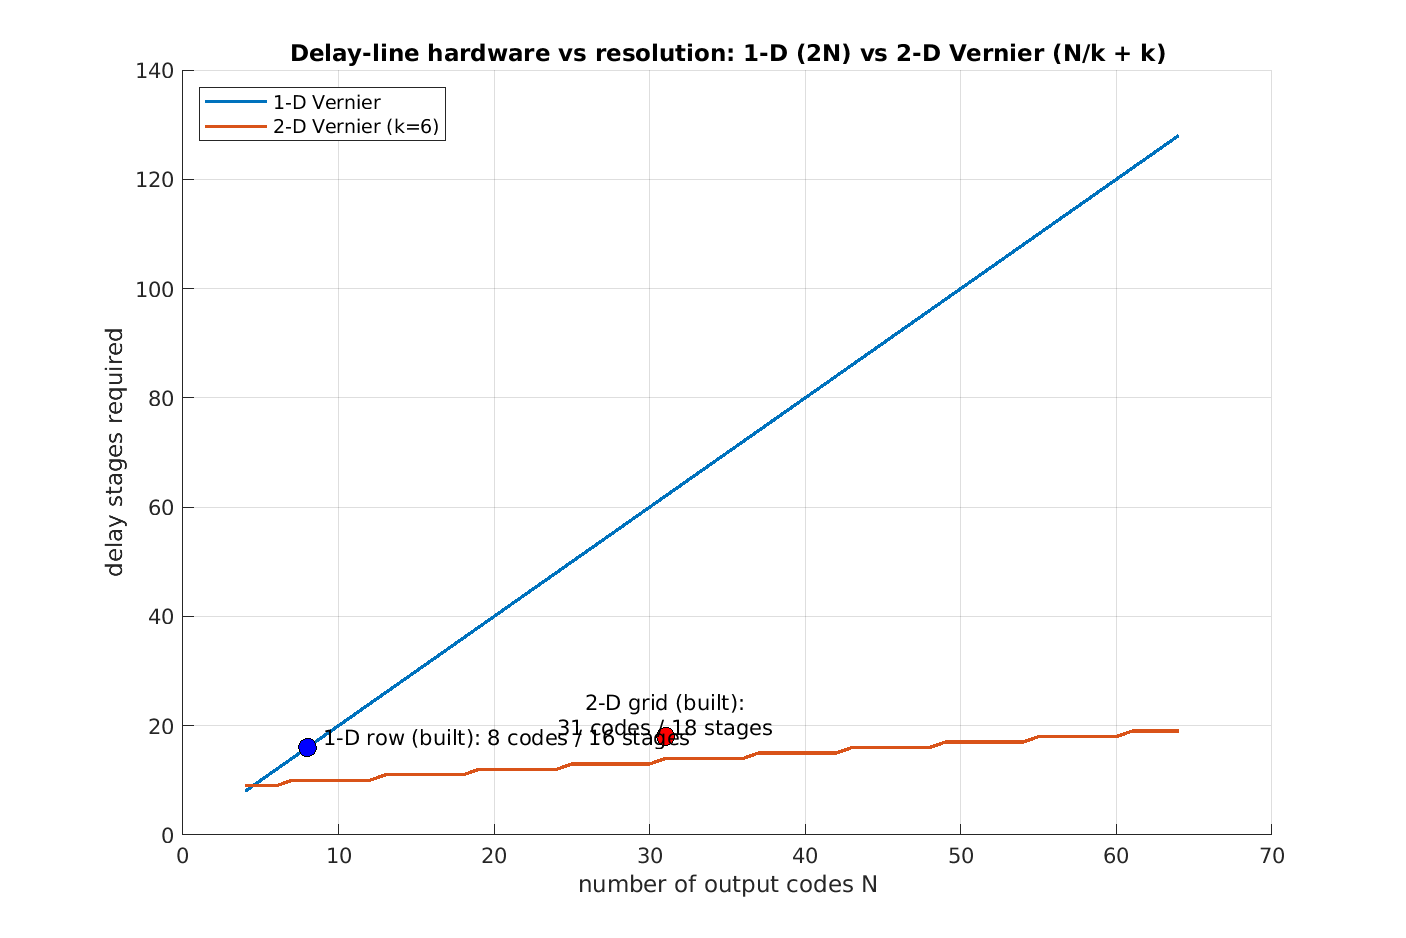
\includegraphics[width=\textwidth]{figures/scaling_1d_vs_2d.png}
  \caption{Delay stages required vs code count, with both built designs
  marked.}
  \label{fig:scaling}
\end{subfigure}\hfill
\begin{subfigure}[t]{0.49\textwidth}
  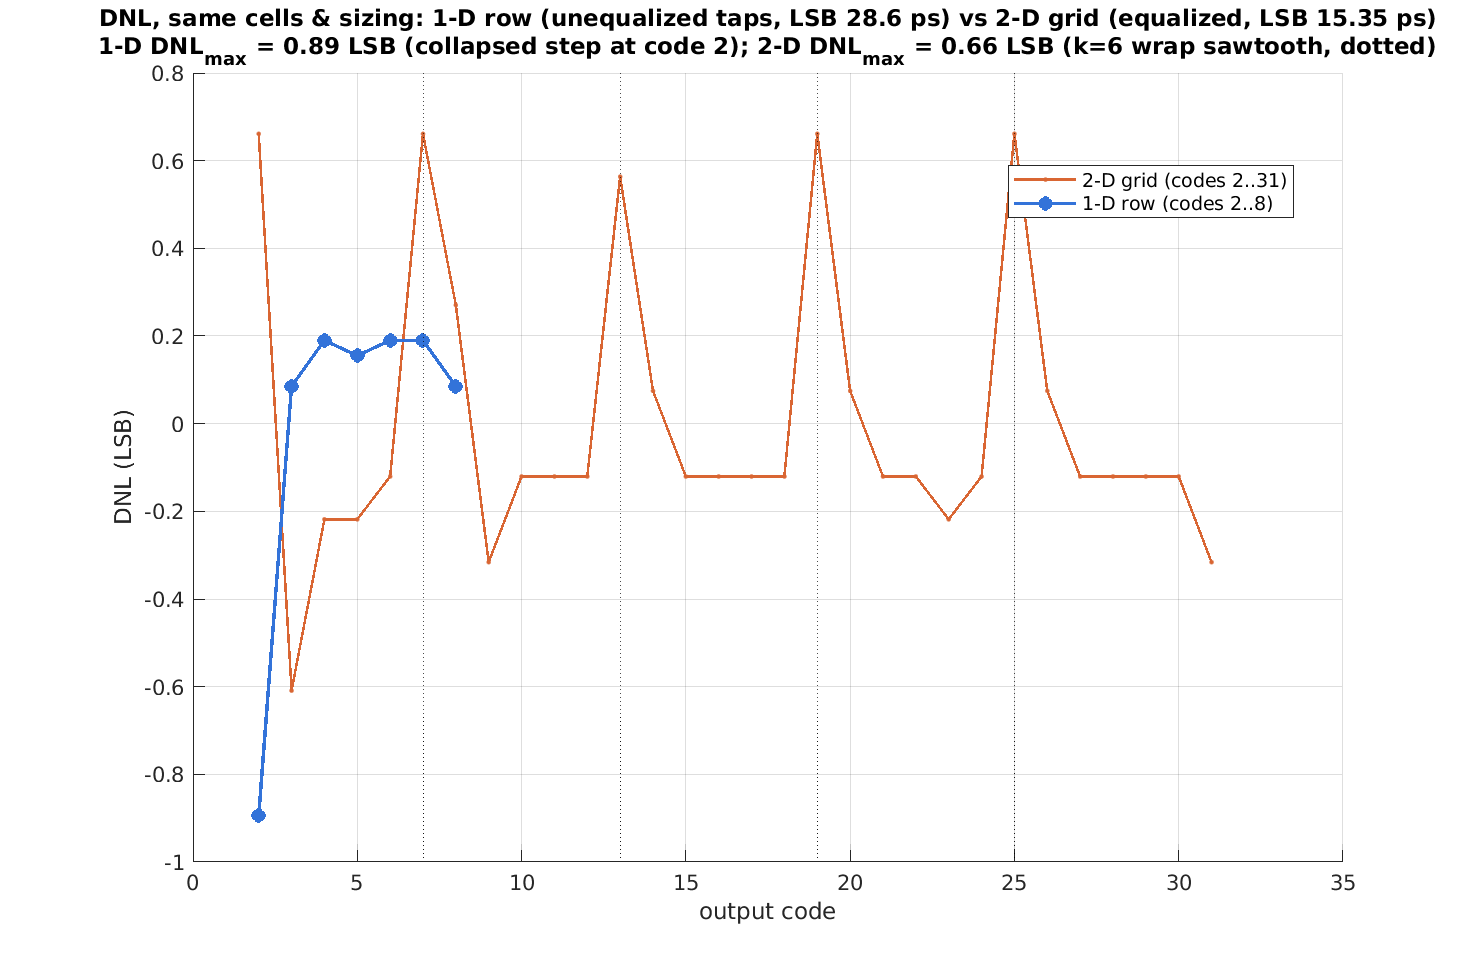
\includegraphics[width=\textwidth]{figures/dnl_1d_vs_2d.png}
  \caption{DNL, 1-D row vs 2-D core, same cells.}
  \label{fig:dnl1d2d}
\end{subfigure}
\caption{Architecture comparison from identical cells (TT).}
\label{fig:1dvs2d}
\end{figure}

To separate the architecture from the circuit design we assembled an 8-code
1-D Vernier row (\texttt{vernier2d/vernier1d\_row}) from the same delay and
latch cells, with trim banks hardwired on and, deliberately, no fan-out
equalization. Table~\ref{tab:1dvs2d} compares the measurements. The row
resolves \SI{28.6}{\pico\second} where the stage-level prediction was
\SI{16.6}{\pico\second}, confirming the loading analysis of
Section~\ref{sec:loading}, and the 2-D core is about twice as area-efficient
per code at comparable energy. Scaled to the full 31 codes, the row would
need $3.4\times$ the delay stages, $1.9\times$ the width and
\SI{3.3}{\nano\second} of full-scale latency against \SI{0.9}{\nano\second}
for the grid.

\begin{table}[H]
\centering
\small
\caption{Measured 1-D row vs 2-D core, identical cells (TT,
\SI{27}{\celsius}).}
\label{tab:1dvs2d}
\begin{tabular}{l c c}
\toprule
 & \textbf{1-D row (built)} & \textbf{2-D core (built)} \\
\midrule
Codes & 8 & 31 \\
LSB & \SI{28.6}{\pico\second} & \SI{15.35}{\pico\second} \\
DNL$_{\max}$ & 0.89 LSB & 0.66 LSB \\
Delay stages & 16 & 18 \\
$\sumw$ per code & \SI{81.4}{\micro\meter} & \SI{42.1}{\micro\meter} \\
Energy per code & \SI{0.33}{\pico\joule} & \SI{0.38}{\pico\joule} \\
Full-scale latency (31 codes) & \SI{3.3}{\nano\second} & \SI{0.9}{\nano\second} \\
\bottomrule
\end{tabular}
\end{table}
